\documentclass[10pt,a4paper]{article}
\usepackage[top=3cm,bottom=4cm,left=3.5cm,right=3.5cm]{geometry}
\usepackage{amsmath,amsthm,amsfonts,amssymb,amscd}
\usepackage{fancyhdr,color,comment,graphicx,environ,float,mathtools,mathrsfs,bbm,listings}
\newcommand{\norm}[1]{\left\lVert#1\right\rVert}

% Custom headers
\pagestyle{fancy}
\lhead{ECON - 8050}
\chead{}
\rhead{Tate Mason}
\lfoot{}
\cfoot{Homework 5}
\rfoot{\thepage}

\begin{document}

\title{Homework 5}
\author{ECON 8050: Macroeconomics II \\ Tate Mason}
\date{}
\maketitle

\includegraphics*[width=\textwidth]{100-a.png}

\includegraphics*[width=\textwidth]{80-a.png} 

\includegraphics*[width=\textwidth]{100-b.png}

\includegraphics*[width=\textwidth]{80-b.png}

\includegraphics*[width=\textwidth]{100-c.png} 

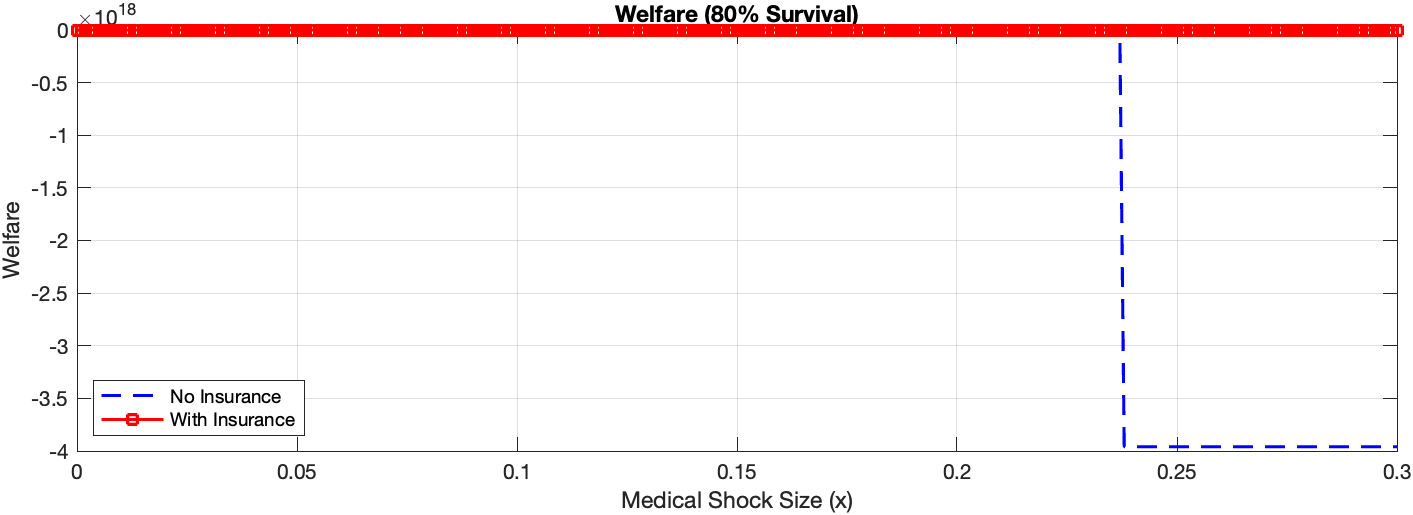
\includegraphics[width = \textwidth]{80-c.png}

\begin{lstlisting}
%% PS5 - OLG
clear;
clc;

%% Setting parameters
alpha = 0.3;
sigma = 3;
beta = 0.99;
pi = 0.1;
n = 0.01;

% Set X Values and Tolerances
xgrid = 0:0.001:0.3;
tol = 1e-5;
maxiter = 10000

%% Creating Variable Arrays
k_no_100 = zeros(size(xgrid));
k_with_100 = zeros(size(xgrid));

w_no_100 = zeros(size(xgrid));
w_with_100 = zeros(size(xgrid));

welf_no_100 = zeros(size(xgrid));
welf_with_100 = zeros(size(xgrid));

% Arrays for survival risk
surv = 0.8;
k_no_80 = zeros(size(xgrid));
k_with_80 = zeros(size(xgrid));

w_no_80 = zeros(size(xgrid));
w_with_80 = zeros(size(xgrid));

welf_no_80 = zeros(size(xgrid));
welf_with_80 = zeros(size(xgrid));

%% Case 1: 100% Survive
for i = 1:length(xgrid)
  x = xgrid(i);
  fprintf('Processing x = %,3f\n', x);
  
  % No Insurance Case
  k = 0.1;
  iter = 0;

  while iter < maxiter
    iter = iter + 1;
    
    r = alpha*k^(alpha-1);
    w = (1-alpha)*k^(alpha);

    risk_premium = 1 + pi*(x/(k*(1+n)))^2;
    s = w/(1+(beta*(1+r)*risk_premium)^(1-sigma));

    k_new = s/(1+n);
    if abs(k_new - k) < tol
      break;
    end
    k = 0.5*k + 0.5*k_new;
  end

  r = alpha*k^(alpha-1)-1;
  w = (1-alpha)*k^alpha;
  c_y = w-k*(1+n);
  c_o_h = (1+r)*k*(1+n);
  c_o_l = max(1e-10, c_o_h-x); 

  welf = c_y^(1-sigma)/(1-sigma) + beta*(pi*c_o_l^(1-sigma)/(1-sigma) + (1-pi)*c_o_h^(1-sigma)/(1-sigma));

  k_no_100(i) = k;
  w_no_100(i) = w;
  welf_no_100(i) = min(0, welf); 
  % Insurance Case
  k = 0.1;
  iter = 0;

  while iter < maxiter
    iter = iter+1;
    
    r = alpha*k^(alpha-1);
    w = (1-alpha)*k^(alpha);

    premium = pi*x/(1+r);
    s = (w-premium)/(1+(beta*(1+r))^(-1/sigma));

    k_new = (s+premium)/(1+n);
    if abs(k_new - k) < tol
      break;
    end
    k = 0.5*k + 0.5*k_new;
  end
  r = alpha * k^(alpha-1);
  w = (1-alpha) * k^alpha;
  premium = pi * x / (1+r);
  c_y = w - premium - k * (1+n);  
  c_o = (1+r) * k * (1+n); 
  welf = c_y^(1-sigma)/(1-sigma) + beta*c_o^(1-sigma)/(1-sigma);

  k_with_100(i) = k;
  w_with_100(i) = w;
  welf_with_100(i) = welf;
end

%% Case 2: Survival Risk
for i = 1:length(xgrid)
  x = xgrid(i);
  fprintf('Processing x = .3%f\n', x);

  k = 0.1;
  transfer = 0;
  iter = 0;

  while iter < maxiter
    iter = iter + 1;
    r = alpha*k^(alpha-1);
    w = (1-alpha)*k^(alpha);
  
    risk_premium = 1 + pi*(x/(k*(1+n)/surv))^2;
    s = (w+transfer)/(1+(beta*surv*(1+r)*risk_premium)^(-1/sigma));

    k_new = surv*s/(1+n);
  
    new_transfer = (1-surv)*s/(1+n);
    transfer = 0.7*transfer + 0.3*new_transfer;

    if abs(k_new - k) < tol
      break;
    end
    k = 0.5*k + 0.5*k_new;
  end
  r = alpha * k^(alpha-1) - 1;
  w = (1-alpha) * k^alpha;
  c_y = w + transfer - k * (1+n) / surv;
  c_o_h = (1+r)*k*(1+n)/surv;
  c_o_l = max(1e-10, c_o_h - x);

  welf = c_y^(1-sigma)/(1-sigma) + beta*surv*(pi*c_o_l^(1-sigma)/(1-sigma) + (1-pi)*c_o_h^(1-sigma)/(1-sigma));
  k_no_80(i) = k;
  w_no_80(i) = w;
  welf_no_80(i) = min(5,welf);

  % With Insurance
  k = 0.1;
  transfer = 0;
  iter = 0;
  
  while iter < maxiter
    iter = iter+1;
    r = alpha*k^(alpha-1);
    w = (1-alpha)*k^(alpha);

    premium = pi*x/((1+r)*surv);
    
    s = (w+transfer-premium)/(1+ (beta*surv*(1+r))^(-1/sigma));

    k_new = (surv*s+premium)/(1+n);

    new_transfer = (1-surv)*s/(1+n);
    transfer = 0.7*transfer + 0.3*new_transfer;

    if abs(k_new-k) < tol
      break;
    end

    k = 0.5*k + 0.5*k_new;
  end
    
    r = alpha * k^(alpha-1) - 1;
    w = (1-alpha) * k^alpha;
    premium = pi * x / ((1+r) * surv);
    c_y = w + transfer - premium - k * (1+n) / surv + premium;
    c_o = (1+r) * k * (1+n) / surv;

    welf = c_y^(1-sigma)/(1-sigma) + beta * surv * c_o^(1-sigma)/(1-sigma);

    k_with_80(i) = k;
    w_with_80(i) = w;
    welf_with_80(i) = welf;
end

%% Plot results
figure('Position', [100, 100, 800, 800]);

% 100% Survival: Capital per worker
subplot(3, 2, 1);
plot(xgrid, k_no_100, 'b-o', 'LineWidth', 1.5);
hold on;
plot(xgrid, k_with_100, 'r-s', 'LineWidth', 1.5);
title('Capital per Worker (100% Survival)');
xlabel('Medical Shock Size (x)');
ylabel('k');
legend('No Insurance', 'With Insurance', 'Location', 'northwest');
grid on;

% 80% Survival: Capital per worker
subplot(3, 2, 2);
plot(xgrid, k_no_80, 'b-o', 'LineWidth', 1.5);
hold on;
plot(xgrid, k_with_80, 'r-s', 'LineWidth', 1.5);
title('Capital per Worker (80% Survival)');
xlabel('Medical Shock Size (x)');
ylabel('k');
legend('No Insurance', 'With Insurance', 'Location', 'northwest');
grid on;

% 100% Survival: Wage
subplot(3, 2, 3);
plot(xgrid, w_no_100, 'b-o', 'LineWidth', 1.5);
hold on;
plot(xgrid, w_with_100, 'r-s', 'LineWidth', 1.5);
title('Wage (100% Survival)');
xlabel('Medical Shock Size (x)');
ylabel('w');
legend('No Insurance', 'With Insurance', 'Location', 'northwest');
grid on;

% 80% Survival: Wage
subplot(3, 2, 4);
plot(xgrid, w_no_80, 'b-o', 'LineWidth', 1.5);
hold on;
plot(xgrid, w_with_80, 'r-s', 'LineWidth', 1.5);
title('Wage (80% Survival)');
xlabel('Medical Shock Size (x)');
ylabel('w');
legend('No Insurance', 'With Insurance', 'Location', 'northwest');
grid on;

% 100% Survival: Welfare
subplot(3, 2, 5);
plot(xgrid, welf_no_100, 'b-o', 'LineWidth', 1.5);
hold on;
plot(xgrid, welf_with_100, 'r-s', 'LineWidth', 1.5);
title('Welfare (100% Survival)');
xlabel('Medical Shock Size (x)');
ylabel('Welfare');
legend('No Insurance', 'With Insurance', 'Location', 'southwest');
grid on;

% 80% Survival: Welfare
subplot(3, 2, 6);
plot(xgrid, welf_no_80, 'b-o', 'LineWidth', 1.5);
hold on;
plot(xgrid, welf_with_80, 'r-s', 'LineWidth', 1.5);
title('Welfare (80% Survival)');
xlabel('Medical Shock Size (x)');
ylabel('Welfare');
legend('No Insurance', 'With Insurance', 'Location', 'southwest');
grid on;
\end{lstlisting}
\end{document}
